% !TeX root = ТеорияОтображений.tex

\chapter{Отображения}
\section{Терминология}
\begin{definition}\label{def:map}
Отображением множества $A$ в множество $B$ называется сопоставление каждому элементу $A$, ровно одного элемента $B$.

Почти всегда одновременно речь будет идти про несколько разных отображений, поэтому принято давать им обозначения в виде букв, например  $f,\,g,\,\varphi,\,\Gamma$ и тд.

Фраза 'Отображение $f$ множества $A$ в множество $B$' на математическом языке записывается как $f:A\rightarrow B$.
\end{definition}
Если отображение $f$ сопоставляет элементу $d$ элемент $v$, то это можно обозначить двумя способами:
\[d\mapsto v\text{ или } v=f(d)\]
первый способ прост для понимания и удобен когда мы хотим сказать что $d$ переходит в $v$. Второй способ изпользует название отображения и удобен когда в рассуждениях фигурируют несколько отображений.

\bigskip
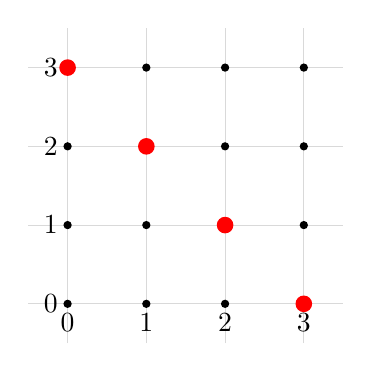
\begin{tikzpicture}

% сетка
\draw[gray!30] (-0.5,-0.5) grid (3.5,3.5);

% подписи осей
\foreach \x in {0,...,3}
  \node[below] at (\x,0) {\x};

\foreach \y in {0,...,3}
  \node[left] at (0,\y) {\y};

% точки
\foreach \x in {0,...,3}{
  \foreach \y in {0,...,3}{
    \ifnum\numexpr\x+\y\relax=3
      \fill[red] (\x,\y) circle (3pt);
    \else
      \fill[black] (\x,\y) circle (1.5pt);
    \fi
  }
}

\end{tikzpicture}

\bigskip
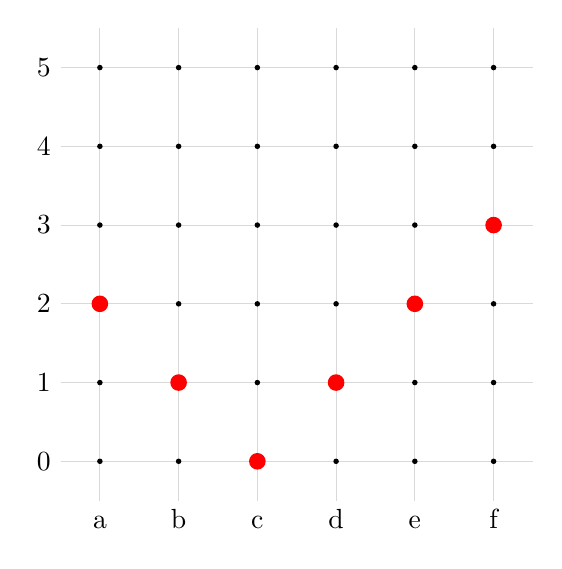
\begin{tikzpicture}
% множества
\def\A{a,b,c,d,e,f}
\def\B{0,1,2,3,4,5}
%сетка
\draw[gray!30] (-0.5,-0.5) grid (5.5,5.5);
%отображение
\foreach \x in {0,...,5}{
  \foreach \y in {0,...,5}{

    \pgfmathparse{abs(\x-2)}

    \ifnum\y=\pgfmathresult
      \fill[red] (\x,\y) circle (3pt);
    \else
      \fill[black] (\x,\y) circle (1pt);
    \fi
  }
}
%координаты
\foreach \x [count=\i] in \A
  \node[below, text height=1.5ex, text depth=.25ex] at (\i-1,-0.5) {\x};
\foreach \y [count=\j] in \B
  \node[left] at (-0.5,\j-1) {\y};
\end{tikzpicture}

\bigskip
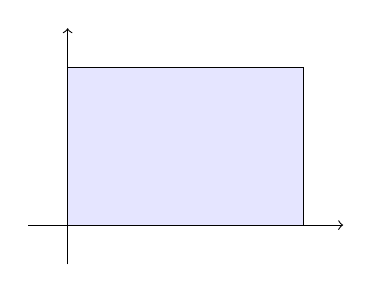
\begin{tikzpicture}
\draw[fill=blue!10] (0,0) rectangle (3,2);
\draw[->] (-0.5,0) -- (3.5,0);
\draw[->] (0,-0.5) -- (0,2.5);
\end{tikzpicture}

\bigskip
\begin{tikzpicture}
\begin{axis}[axis lines=middle]
\addplot[only marks] coordinates {
(1,1) (1,2) (1,3)
(2,1) (2,2) (2,3)
};
\end{axis}
\end{tikzpicture}

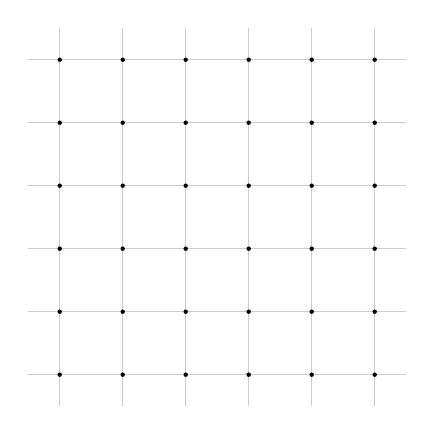
\begin{tikzpicture}[scale=0.8]
%сетка
\draw[gray!40] (-0.5,-0.5) grid (5.5,5.5);
%точки
\foreach \x in {0,...,5}
  \foreach \y in {0,...,5}
    \fill (\x,\y) circle (1pt);
\end{tikzpicture}


определение, примеры, график, 